\documentclass[11pt,fontset=fandol]{ctexart}
\usepackage[a4paper,margin=1in]{geometry}
\usepackage{amsmath,amssymb,amsfonts}
\usepackage{booktabs}
\usepackage{graphicx}
\usepackage{caption}
\usepackage{enumitem}
\usepackage[hidelinks]{hyperref}
\usepackage{xurl}
\usepackage{microtype}
\usepackage{array}
\usepackage[table]{xcolor}

\title{二维单 Target 窗口分布量解释报告\\\large Occupancy Share 与 Ever-Visit Probability 的区别}
\author{}
\date{}

\setlist{nosep}
\setlength{\textfloatsep}{8pt plus 2pt minus 2pt}
\setlength{\floatsep}{6pt plus 2pt minus 2pt}
\setlength{\intextsep}{6pt plus 2pt minus 2pt}
\setlength{\abovecaptionskip}{4pt}
\setlength{\belowcaptionskip}{0pt}
\setlength{\tabcolsep}{5pt}
\renewcommand{\arraystretch}{1.10}

\begin{document}
\maketitle

\section*{结论先行}
本说明稿现在采用一个更温和的 corridor-only 变体来解释同一个问题：为什么在单 target 几何里，\texttt{target funnel} 的占比不是 $100\%$，即使所有轨迹最终都必须经过它。

结论分成两句：
\begin{enumerate}
  \item 现有图里的比例是 \textbf{window-conditioned occupancy share}，它衡量的是“吸收前在某区域停留了多少时间”。
  \item 你直觉里的“所有轨迹都要经过 funnel”对应的是 \textbf{ever-visit probability}，它衡量的是“是否曾经经过该区域”。
\end{enumerate}
这两个量都对，但它们不是同一个 observable，所以数值不需要相等。

\section{几何与区域划分}
本报告沿用 \texttt{grid2d\_one\_two\_target\_gating} 里的对称单 target 几何，但把驱动改成一个更温和的 corridor-only soft-bias variant：
\[
L_x=60,\qquad W_y=15,\qquad (x_s,y_s)=(7,7),\qquad (x_t,y_t)=(58,7).
\]
corridor 带是 $y=5,\dots,9$，两条半透膜位于 corridor 与 outer reservoir 的上下界面，膜 span 为 $x=5,\dots,54$。本说明稿不再画 gate 线，只保留区域划分。为了让颜色和区域能直接一眼对上，下面两张主图都会把同一张配置示意图直接放在主图上方，而不是让读者翻页回看。

这一基线里与 corridor 动力学直接相关的参数也固定如下：
\begin{itemize}
  \item corridor halfwidth 为 $2$，所以中线是 $y=7$，corridor 恰好是 $y=5,\dots,9$；
  \item wall margin 为 $5$，因此两条半透膜只覆盖 $x=5,\dots,54$，也就是上下界面上的 $(x,4)\leftrightarrow(x,5)$ 与 $(x,9)\leftrightarrow(x,10)$；
  \item corridor 内部所有格点都带有\textbf{局部东向偏置}，方向都是 \texttt{E}；
  \item 在膜 span 内，也就是 $5 \le x \le 54$ 时，局部偏置强度改为较温和的 $\delta_{\mathrm{core}}=0.8$；
  \item 在 corridor 的左右开口段，也就是 $x<5$ 或 $x>54$ 时，局部偏置强度取 $\delta_{\mathrm{open}}=0.0$，也就是这些开口段不再额外右推；
  \item 上下 outer reservoir 本来就没有局部右向偏置；这次修改后，真正带局部右推的只剩下主通道段 $5 \le x \le 54,\ 5 \le y \le 9$；
  \item 该变体仍然叠加一个\textbf{全局左向偏置} $(b_x,0)=(-0.08,0)$，因此除主通道段外，其余位置都只感受到这层较弱的向左背景漂移；
  \item 对称膜通透率取 $kappa_{c\to o}=kappa_{o\to c}=0.002$；
  \item 构造转移矩阵时使用的惰性参数为 $q=0.8$。
\end{itemize}
这里有一个容易混淆但很重要的点：主通道里的局部偏置是\emph{向右}的，而全局偏置是\emph{向左}的；双峰结构正是建立在这两层驱动与膜通透受限的共同作用上。我们额外做过 exact 扫描：当 $\delta_{\mathrm{open}}=0$ 固定后，$\delta_{\mathrm{core}}\le 0.6$ 时双峰会塌掉；$\delta_{\mathrm{core}}=0.8$ 是一个折中值，既不再像 $\delta=1$ 那样“把 stay 全部推给右移”，又还能保留可见的双峰。

\section{Peak1, Valley, Peak2 是怎么定义的}
这三个名字不是人工目测出来的，而是 repo 里统一的 exact 规则。

\subsection{先找两个可信的峰}
对 total first-passage pmf \(f(t)\)，代码先取一个长度为 \(7\) 的平滑包络，然后用 \texttt{find\_two\_peaks} 找两处可信局部峰。这里不是只要求“局部最大”，还要求：
\begin{itemize}
  \item 峰高至少达到全局最大值的 \(6\%\)；
  \item 两峰至少相隔 \(20\) 个时间步；
  \item 两个峰之间必须出现真正的 valley，而不是一个小肩峰；
  \item 两峰不能极度失衡，弱峰不能太弱；
  \item valley 相对峰顶必须有可见的下降。
\end{itemize}
所以 \texttt{peak1} 和 \texttt{peak2} 的中心其实是两个“通过可信性筛选的峰位置”，不是肉眼随便挑出来的点。

\subsection{再在两峰之间取 valley}
如果找到两个可信峰，代码就在它们之间的平滑曲线上取最小值位置
\[
t_{\mathrm{valley}}=\arg\min_{t\in[t_{\mathrm{peak1}},\,t_{\mathrm{peak2}}]} f_s(t),
\]
其中 \(f_s\) 是平滑后的曲线。于是：
\begin{itemize}
  \item \texttt{peak1} 的中心是 \(t_{\mathrm{peak1}}\)；
  \item \texttt{valley} 的中心是 \(t_{\mathrm{valley}}\)；
  \item \texttt{peak2} 的中心是 \(t_{\mathrm{peak2}}\)。
\end{itemize}

\subsection{窗口宽度怎么取}
窗口本身不是自由手调的，而是按
\[
\mathrm{half}=\max\!\left(8,\ \min\!\left(26,\ \left\lfloor\frac{t_{\mathrm{peak2}}-t_{\mathrm{peak1}}}{7}\right\rfloor\right)\right)
\]
统一取半宽，然后对三个中心都用同一个半宽：
\[
[t_{\mathrm{peak1}}-\mathrm{half},\ t_{\mathrm{peak1}}+\mathrm{half}],
\quad
[t_{\mathrm{valley}}-\mathrm{half},\ t_{\mathrm{valley}}+\mathrm{half}],
\quad
[t_{\mathrm{peak2}}-\mathrm{half},\ t_{\mathrm{peak2}}+\mathrm{half}].
\]

对当前这组 corridor-only soft 变体，exact 结果是
\[
t_{\mathrm{peak1}}=554,\qquad t_{\mathrm{valley}}=1490,\qquad t_{\mathrm{peak2}}=2327.
\]
因为 \(t_{\mathrm{peak2}}-t_{\mathrm{peak1}}=1773\)，所以上式仍然给出 \(\mathrm{half}=26\)。因此当前报告里实际使用的三个窗口就是
\[
\texttt{peak1}=[528,580],\qquad
\texttt{valley}=[1464,1516],\qquad
\texttt{peak2}=[2301,2353].
\]

\subsection{这和 phase 判据的关系}
要注意，窗口定义和“是不是 clear double peak”是两回事。窗口只负责在三个代表时段里取样；而 phase 判据另外还会检查两峰是否真的分得开。在 one-target canonical 规则里，核心是：
\begin{itemize}
  \item \texttt{find\_two\_peaks} 必须先找到两个可信峰；
  \item 分离度 \(\mathrm{sep}_{\mathrm{peaks}}\) 需要满足 \(\mathrm{sep}_{\mathrm{peaks}}\ge 1\) 才算 clear double peak。
\end{itemize}
对当前这个软偏置变体，exact 结果是 \(\mathrm{sep}_{\mathrm{peaks}}\approx 0.675\)。因此它仍然有两个可信峰，但严格说属于 ``has double peak but not clear double peak''，也就是 \texttt{phase=1} 而不是 \texttt{phase=2}。

\section{当前图里到底画的是什么}
\subsection{Window-conditioned occupancy share}
设 $X_t$ 是第 $t$ 步的位置，$T$ 是 first-passage time，$W$ 是一个窗口，例如 \texttt{peak1}、\texttt{valley} 或 \texttt{peak2}。对任意区域 $R$，本轮图里真正画的是
\[
p^{\mathrm{occ}}_W(R)
=
\frac{
\mathbb{E}\!\left[
\mathbf{1}_{\{T\in W\}}
\sum_{t=0}^{T-1}\mathbf{1}_{\{X_t\in R\}}
\right]
}{
\mathbb{E}\!\left[
\mathbf{1}_{\{T\in W\}}\,T
\right]
}.
\]
它的含义是：
\begin{quote}
在所有命中窗口 $W$ 的轨迹里，随机抽取一个“吸收前时刻”，该时刻落在区域 $R$ 的概率。
\end{quote}

所以它是 \textbf{时间加权} 的量。某条轨迹即使必经 funnel，只要在 funnel 里停得很短，它对 occupancy share 的贡献就会很小。

\subsection{为什么 funnel 不会自动变成 $100\%$}
考虑一个极简例子：
\begin{itemize}
  \item 每条轨迹在 corridor 里平均停 $100$ 步；
  \item 然后进入 funnel，只停 $2$ 步就吸收。
\end{itemize}
那么：
\[
p^{\mathrm{visit}}(\texttt{funnel}) = 100\%,
\qquad
p^{\mathrm{occ}}(\texttt{funnel}) \approx \frac{2}{102}\approx 2\%.
\]
也就是说，“一定经过”并不等于“占据时间占大头”。

\section{你直觉里的那个量是什么}
\subsection{Ever-visit probability}
如果我们关心的是
\begin{quote}
命中窗口 $W$ 的轨迹里，有多少条轨迹在吸收前 \emph{曾经到过} 区域 $R$？
\end{quote}
那么对应量是
\[
p^{\mathrm{visit}}_W(R)
=
\mathbb{P}\!\left(\exists t<T:\ X_t\in R \,\middle|\, T\in W\right).
\]
这才是路径事件概率，而不是时间占据比例。

对于本几何下的 \texttt{target funnel}，exact 计算给出的就是
\[
p^{\mathrm{visit}}_{\texttt{peak1}}(\texttt{funnel})
=
p^{\mathrm{visit}}_{\texttt{valley}}(\texttt{funnel})
=
p^{\mathrm{visit}}_{\texttt{peak2}}(\texttt{funnel})
=1.
\]
也就是说，你关于“所有轨迹都必须经过 funnel”的直觉是对的；只不过它对应的是 \textbf{ever-visit}，而不是当前主图里的 \textbf{occupancy share}。

\section{两种量的直接对照}
下面这两幅主图我都保留，而且连续放置，不让别的图表打断阅读顺序。建议的阅读方式是：先看图~\ref{fig:overview}，理解“时间主要耗在哪里”；再紧接着看图~\ref{fig:profile-bars}，判断“如果只看路径事件，区域排序会不会改写”。

\begin{figure}[!htbp]
  \centering
  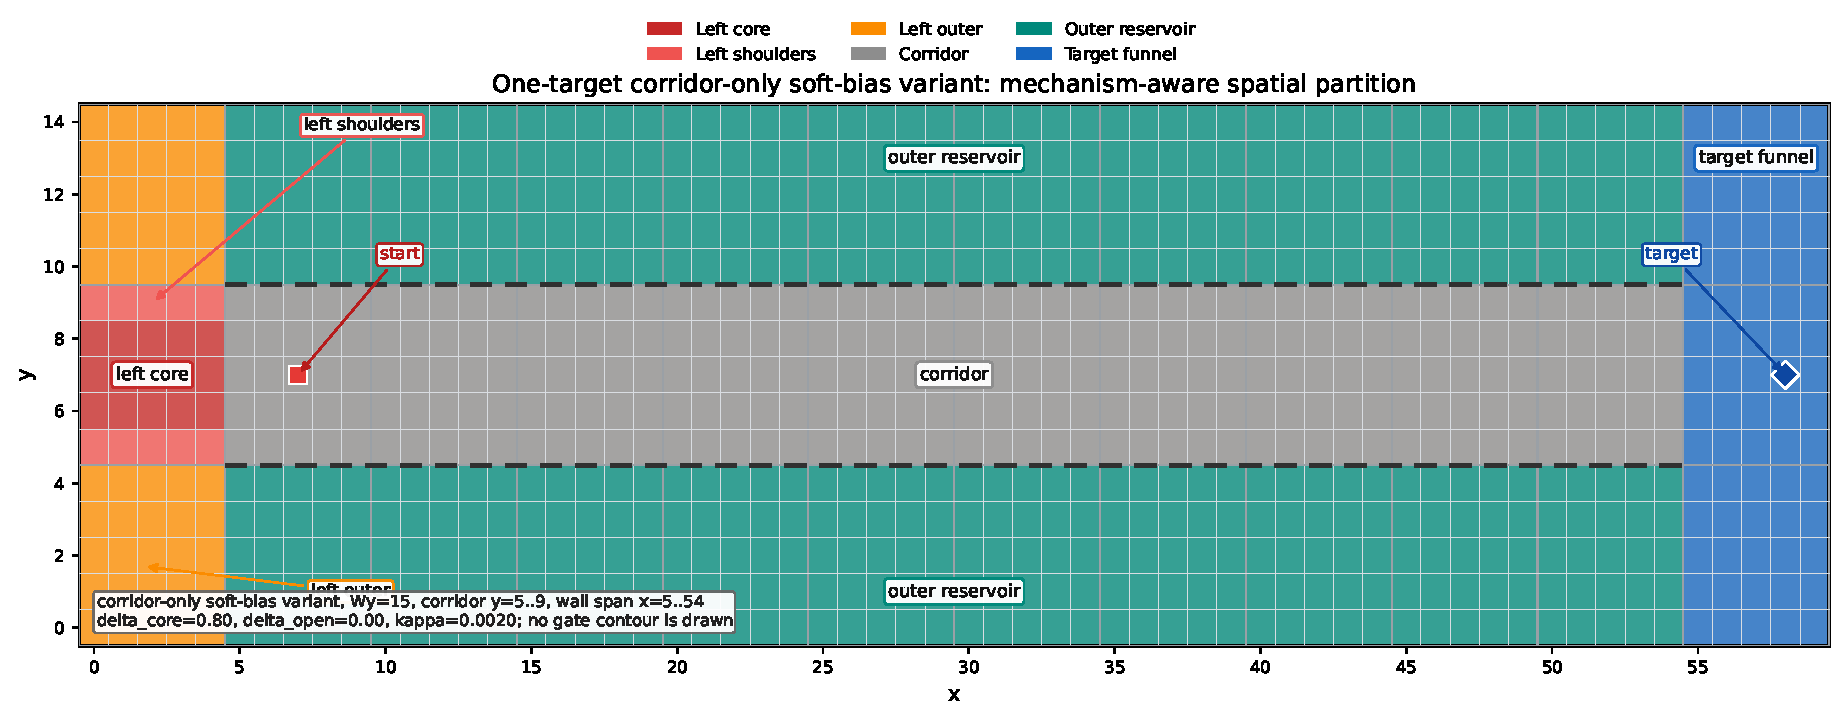
\includegraphics[width=0.92\linewidth]{../artifacts/figures/one_target_partition.pdf}

  \vspace{0.35em}
  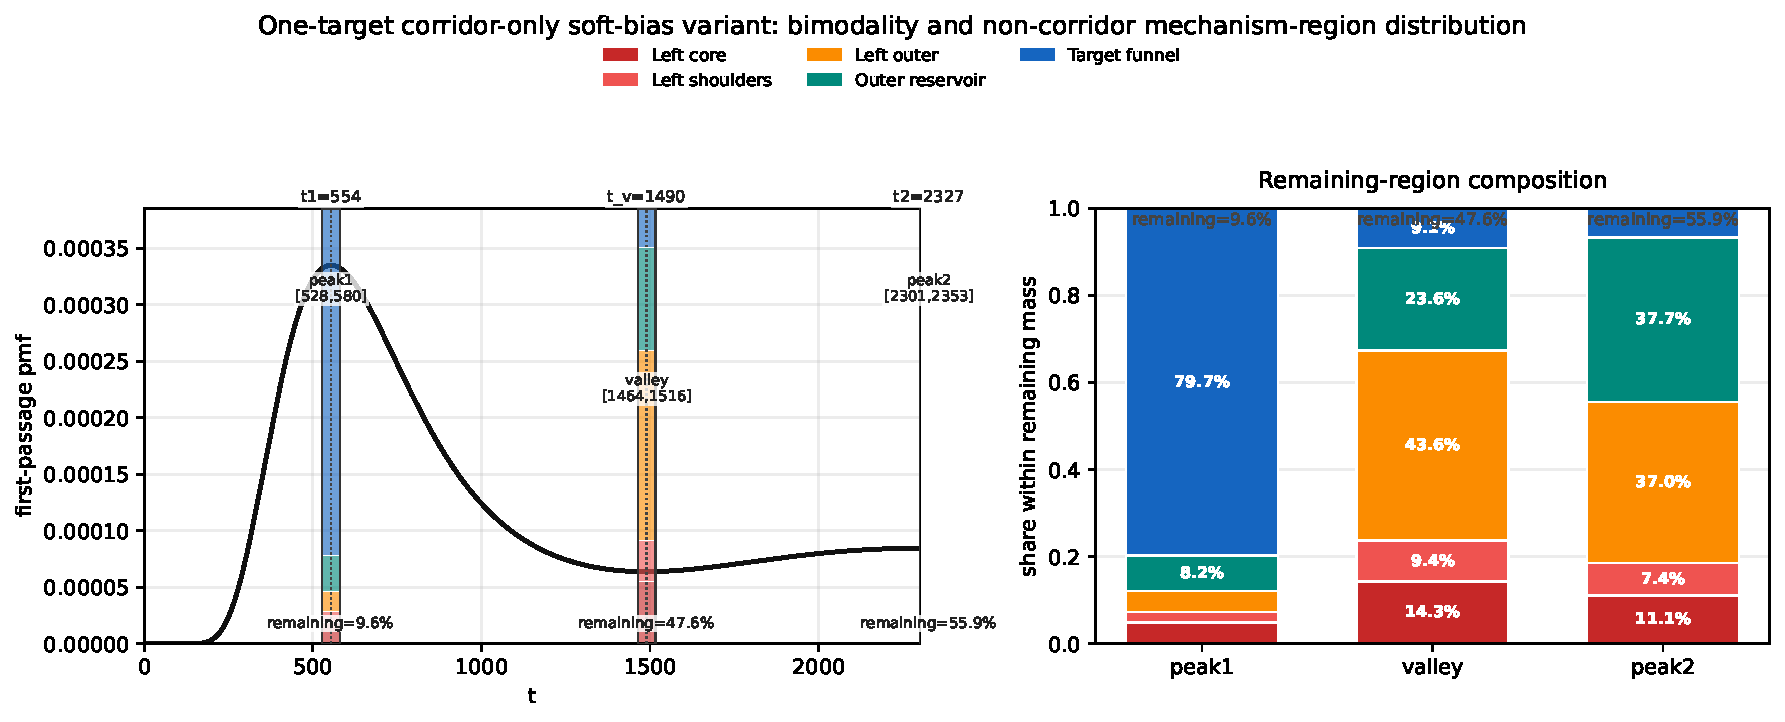
\includegraphics[width=0.98\linewidth]{../artifacts/figures/one_target_bimodal_non_corridor.pdf}
  \caption{第一张主图的总览布局。上：corridor-only soft 变体的机制区域划分。这里保留完整空间：\texttt{left core}、\texttt{left shoulders}、\texttt{left outer}、\texttt{corridor}、\texttt{outer reservoir}、\texttt{target funnel}。下：occupancy 主图，exact 双峰曲线上直接叠加的 full-height window composition bars。每个窗口条覆盖自己的时间范围，条内颜色表示去掉 \texttt{corridor} 后剩余质量的组成；右侧柱图给出同样组成的独立显示。这样颜色和区域可以一眼对照。}
  \label{fig:overview}
\end{figure}

先把图~\ref{fig:overview} 看成“时间分布版”：它告诉我们，在命中同一个窗口的轨迹里，吸收前的大部分时间到底花在了哪些非 corridor 区域。

\begin{figure}[!htbp]
  \centering
  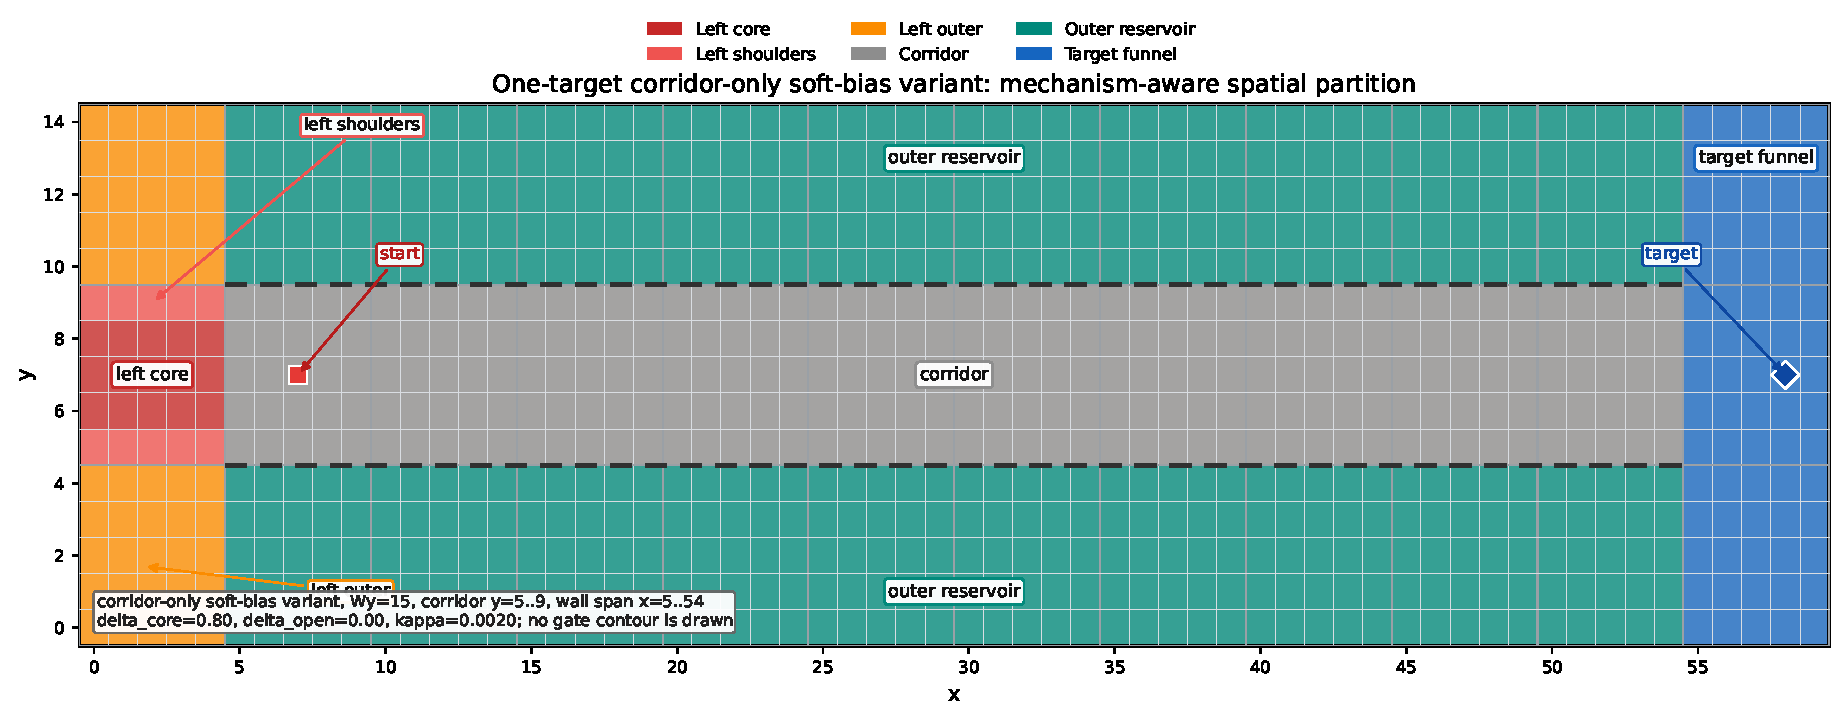
\includegraphics[width=0.92\linewidth]{../artifacts/figures/one_target_partition.pdf}

  \vspace{0.35em}
  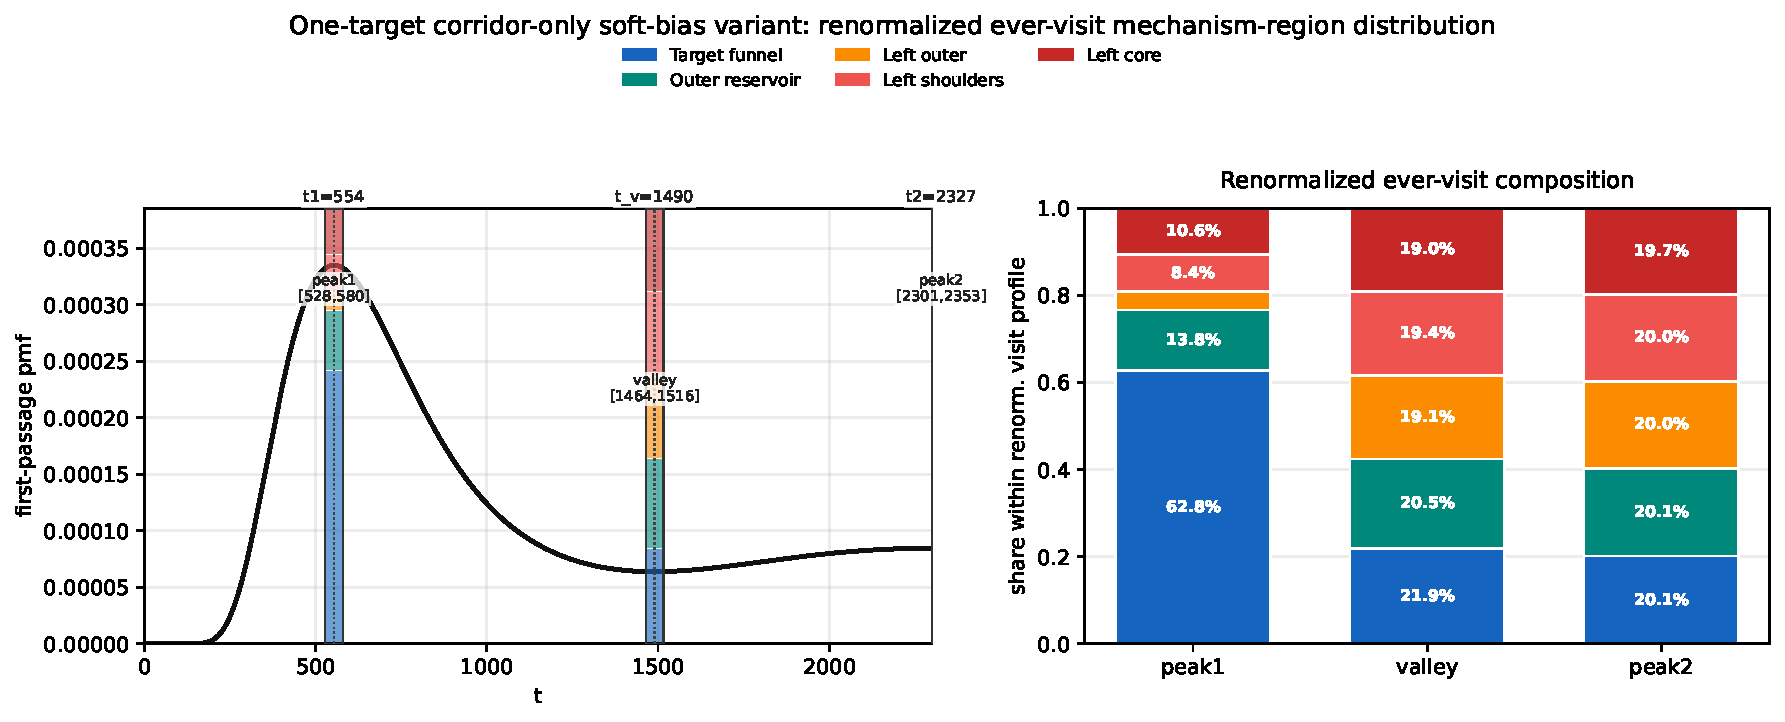
\includegraphics[width=0.98\linewidth]{../artifacts/figures/one_target_ever_visit_non_corridor.pdf}
  \caption{第二张主图也采用同样的总览布局，把配置示意图直接放在 ever-visit 主图上方。下图与图~\ref{fig:overview} 的下半部分使用相同的双峰曲线和同一组窗口，但把区域权重换成 ever-visit 的归一化 profile。右侧柱图画出各窗口下的 renormalized ever-visit composition。这里必须强调：它不是 raw ever-visit probability 的直接堆叠，而是为了和 occupancy 图做版式一致、形状可比而做的归一化。}
  \label{fig:profile-bars}
\end{figure}

\begin{figure}[!htbp]
  \centering
  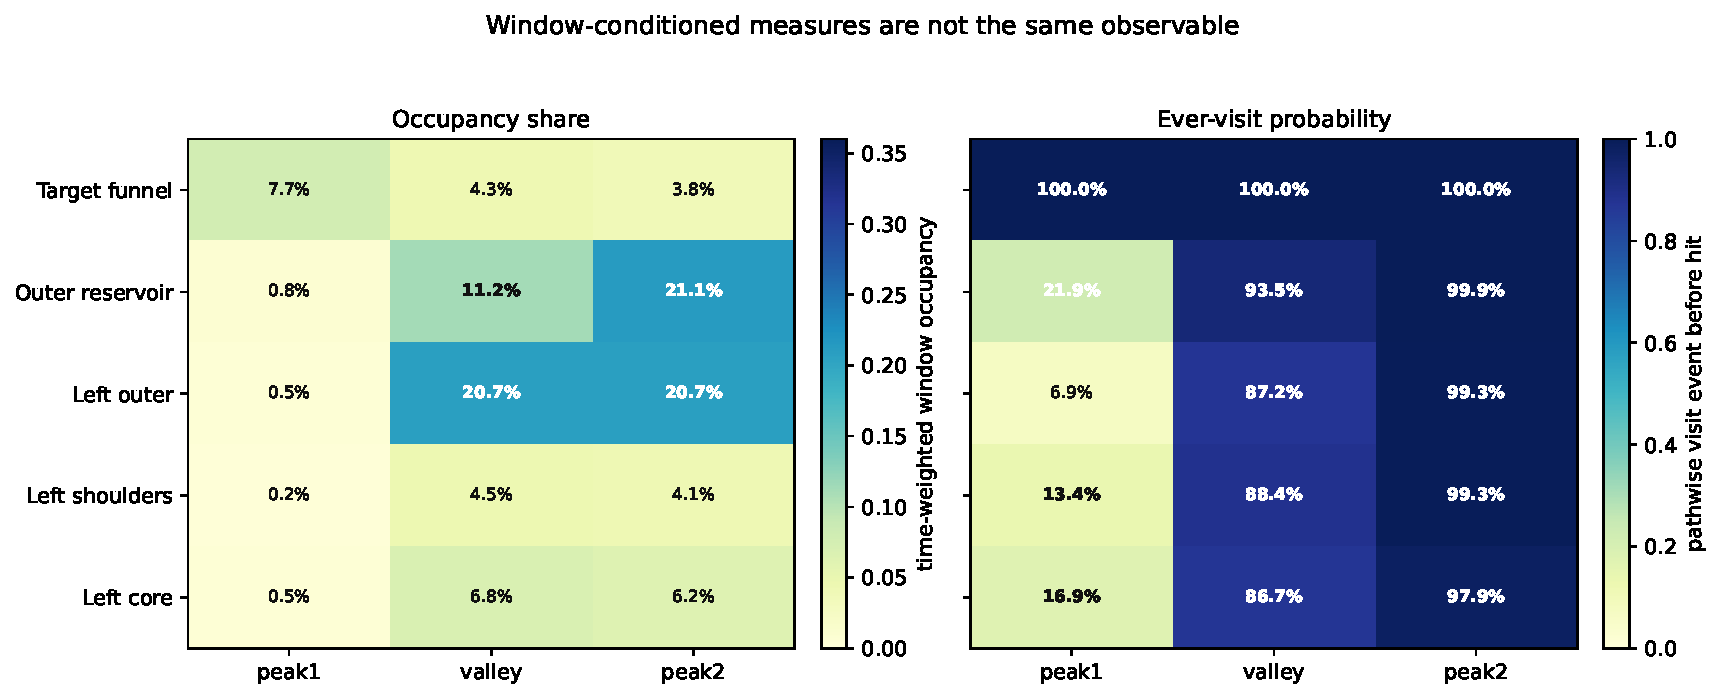
\includegraphics[width=0.92\linewidth]{../artifacts/figures/window_measure_comparison.pdf}
  \caption{左图是 occupancy share，右图是 ever-visit probability。最关键的一行是 \texttt{target funnel}：occupancy share 只有约 $7.7\% / 4.3\% / 3.8\%$，但 ever-visit 在三个窗口里都是 $100\%$。这正是“停留时间”和“是否经过”两个 observable 的差别。}
  \label{fig:measure-compare}
\end{figure}

\begin{table}[!htbp]
  \centering
  \footnotesize
  \begin{tabular}{lcccccc}
\toprule
Region & Occ. p1 & Visit p1 & Occ. valley & Visit valley & Occ. p2 & Visit p2 \\
\midrule
Target funnel & 7.7\% & 100.0\% & 4.3\% & 100.0\% & 3.8\% & 100.0\% \\
Outer reservoir & 0.8\% & 21.9\% & 11.2\% & 93.5\% & 21.1\% & 99.9\% \\
Left outer & 0.5\% & 6.9\% & 20.7\% & 87.2\% & 20.7\% & 99.3\% \\
Left shoulders & 0.2\% & 13.4\% & 4.5\% & 88.4\% & 4.1\% & 99.3\% \\
Left core & 0.5\% & 16.9\% & 6.8\% & 86.7\% & 6.2\% & 97.9\% \\
\bottomrule
\end{tabular}

  \caption{各窗口下 occupancy share 与 ever-visit probability 的 exact 对照。}
  \label{tab:measure-compare}
\end{table}

\begin{table}[!htbp]
  \centering
  \footnotesize
  \begin{tabular}{lcc}
\toprule
Window & Cosine similarity & Total variation distance \\
\midrule
peak1 & 0.9838 & 0.1728 \\
valley & 0.8270 & 0.2758 \\
peak2 & 0.8153 & 0.3461 \\
\bottomrule
\end{tabular}

  \caption{把上图两种 profile 都归一化成同一套 5 区向量之后的相似度。Cosine similarity 越接近 $1$，形状越接近；total variation distance 越小，差异越小。}
  \label{tab:profile-sim}
\end{table}

这里要特别强调：表~\ref{tab:profile-sim} 比较的是两个\emph{归一化 profile} 的形状，而不是拿 raw ever-visit probability 直接做 composition。这个比较只回答“窗口里哪些区域相对更重要时，两种 observable 的排序像不像”，不回答“这些事件概率本身是否可加”。

\section{为什么 Monte Carlo 会和 exact 一致}
\subsection{如果 Monte Carlo 统计的是 occupancy share}
设第 $m$ 条 Monte Carlo 轨迹的首达时间为 $T_m$，轨迹为 $(X_t^{(m)})_{t=0}^{T_m-1}$。那么 occupancy share 的自然 MC 估计量是
\[
\widehat p^{\mathrm{occ}}_W(R)
=
\frac{
\sum_{m=1}^M
\mathbf{1}_{\{T_m\in W\}}
\sum_{t=0}^{T_m-1}\mathbf{1}_{\{X_t^{(m)}\in R\}}
}{
\sum_{m=1}^M
\mathbf{1}_{\{T_m\in W\}}\,T_m
}.
\]
这就是“在命中窗口 $W$ 的轨迹里，把所有吸收前时间点都摊平，再看有多少比例落在 $R$”。当 $M\to\infty$ 时，由大数定律，它会收敛到图中 exact 的 occupancy share。

\subsection{如果 Monte Carlo 统计的是 ever-visit probability}
另一种 MC 估计量是
\[
\widehat p^{\mathrm{visit}}_W(R)
=
\frac{
\sum_{m=1}^M
\mathbf{1}_{\{T_m\in W\}}
\mathbf{1}_{\{\exists t<T_m:\ X_t^{(m)}\in R\}}
}{
\sum_{m=1}^M
\mathbf{1}_{\{T_m\in W\}}
}.
\]
这个量会收敛到 exact 的 ever-visit probability，而不是 occupancy share。

\subsection{所以 MC 和 exact 什么时候“应该相似”？}
答案是：
\begin{itemize}
  \item 如果 MC 估计的是同一个 observable，它就应该和 exact 相似，只差采样噪声。
  \item 如果 MC 估计的是另一个 observable，它当然可以和 exact 图长得完全不一样。
\end{itemize}

在本例里：
\begin{itemize}
  \item 用时间点统计的 MC 会接近图中的 occupancy share；
  \item 用“是否到过”统计的 MC 会给出 \texttt{target funnel} 约等于 $100\%$。
\end{itemize}

\section*{总结}
本报告的核心不是重新发现一个机制，而是把两个常被混用的量彻底拆开：
\begin{enumerate}
  \item \textbf{occupancy share}：时间加权，问的是“在哪里待得久”；
  \item \textbf{ever-visit probability}：路径事件，问的是“有没有到过那里”。
\end{enumerate}
一旦把这两者分开，\texttt{target funnel} “必经但占比不高” 就不再矛盾，而是完全符合它靠近吸收点、停留时间短的几何直觉。

\end{document}
